\chapter{方势阱中的粒子}\label{chap:square-well}

\section{定态 Schrödinger 方程}\label{sec:square-well-time-independent}

先考察经典粒子在方势阱中的行为.若粒子能量为负,则粒子必须位于势阱中;它以恒定速度运动,直到撞到势阱边缘,随后瞬间从墙壁反射,并以相同速率向相反方向运动.若粒子能量为正,则它始终沿同一方向运动;在势阱外和势阱内,速度分别为不同的常数.

在量子情形中,我们主要关注 Schrödinger 算子的负特征值(\(E<0\))所对应的特征向量.当然,在量子理论中,能量特征向量除一个整体相位因子外不随时间变化.不过,由于能量为负的经典粒子在势阱各部分停留的时间相同,可以预期量子粒子在势阱各部分被发现的概率近似相等.对于“高激发态”,例如图~\ref{fig:square-well-deep-excited} 所示的状态,这一预期确实会实现.但量子粒子在势阱外被发现的概率虽小却非零,而经典粒子不可能出现在那里.

我们的目标是研究定态 Schrödinger 方程,即特征值方程
\begin{equation}
-\frac{\hbar^{2}}{2m}\frac{\mathrm{d}^{2}\psi}{\mathrm{d}x^{2}}
+V(x)\psi(x)=E\psi(x),
\label{eq:square-well-schrodinger}
\end{equation}
其中特征值 \(E\) 和相应特征向量 \(\psi\)(物理学术语称“特征函数”)都尚未确定.作为二阶线性常微分方程,式~\eqref{eq:square-well-schrodinger} 对任意 \(E\) 总有一个二维解空间.不过,我们要找的是属于量子 Hilbert 空间 \(L^{2}(\mathbb{R})\) 的解.实际上只有有限多个 \(E\)(全都满足 \(E<0\))使得式~\eqref{eq:square-well-schrodinger} 在 \(L^{2}(\mathbb{R})\) 中存在非零解.因此,Schrödinger 算子 \(\widehat H\) 在零以下具有离散谱,在零以上具有连续谱.

本节考虑一个简单但有启发性的例子,它可以用初等方法求解.我们在 \(\mathbb{R}^{1}\) 中取势能
\begin{equation}
V(x)=
\begin{cases}
-C,&-A\le x\le A,\\
0,&|x|>A,
\end{cases}
\label{eq:square-well-potential}
\end{equation}
\begin{figure}[htbp]
  \centering
  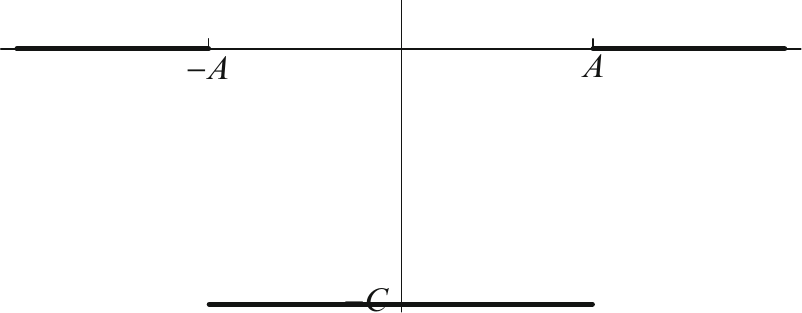
\includegraphics[width=.72\textwidth]{figures/figure-5-1.png}
  \caption{方势阱的势能.}
  \label{fig:square-well-potential}
\end{figure}
其中 \(A,C\) 是正数.区域 \(-A\le x\le A\) 称为势能的“方势阱”(图~\ref{fig:square-well-potential}).

\section{定义域问题与匹配条件}\label{sec:square-well-domain}

在开始求解式~\eqref{eq:square-well-schrodinger} 之前,必须注意 Hamilton 算子的无界性.左端的 Schrödinger 算子
\[
\widehat H=-\frac{\hbar^{2}}{2m}\frac{\mathrm{d}^{2}}{\mathrm{d}x^{2}}+V(X)
\]
是无界算子,即不存在常数 \(C\),使得对所有 \(\psi\) 都有 \(\|\widehat H\psi\|\le C\|\psi\|\),其中范数是 \(L^{2}\) 范数.另一方面,我们希望以某种方式定义 \(\widehat H\),使其为自伴算子.但根据关于无界算子的基本结论,一个定义在整个 Hilbert 空间上的自伴算子必须有界.

因此,\(\widehat H\) 不会定义在整个 Hilbert 空间 \(L^{2}(\mathbb{R})\) 上,而只定义在其中的一个稠密子空间上.实际而言,说 \(\widehat H\) 没有定义在整个 Hilbert 空间上,只是说对于 \(L^{2}(\mathbb{R})\) 中许多函数 \(\psi\),二阶导数 \(\mathrm{d}^{2}\psi/\mathrm{d}x^{2}\) 不存在,或者虽然存在却不属于 \(L^{2}(\mathbb{R})\).在本例中势能 \(V\) 有界,所以只要 \(\psi\in L^{2}(\mathbb{R})\),\(V\psi\) 总属于 \(L^{2}(\mathbb{R})\).

由于方势阱的势能有界,Hamilton 算子 \(\widehat H=P^{2}/(2m)+V(X)\) 的定义域与动能算子 \(P^{2}/(2m)=-(\hbar^{2}/2m)\mathrm{d}^{2}/\mathrm{d}x^{2}\) 的定义域相同.第~9 章将看到,动能算子的定义域可以描述为:那些属于 \(L^{2}(\mathbb{R})\) 且其弱导数(或分布导数,见附录~\ref{app:def:distribution-derivative})\(\mathrm{d}^{2}\psi/\mathrm{d}x^{2}\) 仍属于 \(L^{2}(\mathbb{R})\) 的函数空间.这个条件等价于:存在某个 \(L^{2}\) 函数 \(\phi\),使得 \(\psi\) 是 \(\phi\) 的二重积分(对积分常数作某种选择).

另一方面,由于方势阱的势能是分段常数,式~\eqref{eq:square-well-schrodinger} 的任意解在 \(x=\pm A\) 之外都光滑,并且 \(\psi\) 与 \(\psi'\) 在 \(A\) 和 \(-A\) 处都有左右极限.事实上,在区间 \((-\infty,-A)\)、\((-A,A)\) 和 \((A,\infty)\) 上,解都只是(实或复)指数函数的线性组合.对这种函数,不难判断何时属于 \(\widehat H\) 的定义域.

\begin{proposition}[方势阱的定义域条件]\label{prop:square-well-domain}
设 \(\psi\) 在区间 \((-\infty,-A)\)、\((-A,A)\) 和 \((A,\infty)\) 上分别光滑.那么,\(\psi\) 属于势能函数由式~\eqref{eq:square-well-potential} 给出的 \(\widehat H\) 的定义域,当且仅当:
\begin{enumerate}
\item \(\psi\) 与 \(\mathrm{d}\psi/\mathrm{d}x\) 在 \(x=\pm A\) 处连续;
\item \(\mathrm{d}^{2}\psi/\mathrm{d}x^{2}\) 属于 \(L^{2}(\mathbb{R})\).
\end{enumerate}
\end{proposition}

\begin{proof}
先假设 \(\psi\) 满足 (1) 和 (2).不难看出,\(\psi\) 的分布二阶导数就是在 \(x\ne\pm A\) 处按通常逐点意义计算的 \(\mathrm{d}^{2}\psi/\mathrm{d}x^{2}\)(在 \(x=\pm A\) 这两个测度为零的点,可以不定义二阶导数).因此,以分布意义计算的二阶导数属于 \(L^{2}(\mathbb{R})\).

反过来,如果 \(\psi\) 或 \(\psi'\) 在 \(x=A\) 或 \(x=-A\) 处有间断,那么分布导数将包含这些点处 \(\delta\) 函数的非零倍数,或者 \(\delta\) 函数导数的非零倍数.但 \(\delta\) 函数及其导数都不是平方可积函数.因此必须满足连续性条件.
\end{proof}

来理解 \(\psi\) 和 \(\mathrm{d}\psi/\mathrm{d}x\) 的连续性条件在实际中的含义.由于 \(V\) 在 \((-\infty,-A)\) 上为常数,可以很容易地在该区间求解式~\eqref{eq:square-well-schrodinger};解空间是二维的.一旦从这个解空间中选定一个解,那么当 \(x\) 从左侧趋于 \(-A\) 时,\(\psi\) 和 \(\mathrm{d}\psi/\mathrm{d}x\) 的值就成为在 \((-A,A)\) 上求解方程的初始条件.因此,\(\psi\) 与 \(\psi'\) 的连续性为 \((-\infty,-A)\) 上的解与 \((-A,A)\) 上的解提供了“匹配条件”.不能在 \((-\infty,-A)\) 和 \((-A,A)\) 上任意分别选择解;在边界处,\(\psi\) 和 \(\psi'\) 的值必须匹配.(在具有不连续系数的初等常微分方程中,也会出现同样的匹配条件.)

一旦在 \((-\infty,-A)\) 上选定一个解,就能唯一地把它延拓到 \((-A,A)\);随后在 \(A\) 左侧趋近时 \(\psi,\psi'\) 的值又成为在 \((A,\infty)\) 上求解方程的初始条件.结论是:一旦在 \((-\infty,-A)\) 的二维解空间中选择一个解,就没有额外选择;微分方程与匹配条件给出了把解从 \((-\infty,-A)\) 唯一延拓到整个实轴的方式.

\section{寻找平方可积解}\label{sec:square-well-solutions}

如果 \(E>0\),那么在 \(x<-A\) 的任意解都是两个复指数的线性组合;这样的函数除非恒等于零,否则不可能平方可积.如果我们在 \(x<-A\) 区域令 \(\psi\) 恒等于零,那么连续性条件要求 \(x\to-A^{+}\) 时 \(\psi\) 和 \(\psi'\) 都趋于零.因此 \(-A\) 处的匹配条件迫使 \([-A,A]\) 上的解也恒等于零;最后通过 \(x=A\) 的匹配,得到 \([A,\infty)\) 上的零解.所以,当 \(E>0\) 时,满足命题~\ref{prop:square-well-domain} 连续性条件的任何解都恒等于零.\(E=0\) 时分析相同,此时在 \((-\infty,A]\) 上的解形如 \(c_{1}+c_{2}x\),只有 \(c_{1}=c_{2}=0\) 时才平方可积.

因此,要想得到既平方可积又属于 \(\widehat H\) 定义域的解,必须取 \(E<0\).当 \(E<0\) 时,\((-\infty,-A)\) 上的解是 \(\exp(\alpha x)\) 和 \(\exp(-\alpha x)\) 的线性组合,其中
\begin{equation}
\alpha=\frac{\sqrt{2m|E|}}{\hbar}.
\label{eq:square-well-alpha}
\end{equation}
为了使 \(\psi\) 在 \((-\infty,-A)\) 上平方可积,\(\exp(-\alpha x)\) 的系数必须为零,因为当 \(x\to-\infty\) 时它指数增长.因此该区间上的 \(\psi\) 必为 \(c\exp(\alpha x)\).一旦选定 \(c\),就能通过在 \(x=-A\) 处匹配 \(\psi,\psi'\),唯一地得到 \((-A,A)\) 上的解;再通过 \(x=A\) 处的匹配,唯一地得到 \((A,\infty)\) 上的解.后一个区间上的解又是 \(\exp(\alpha x)\) 与 \(\exp(-\alpha x)\) 的线性组合.为了使它属于 \(L^{2}\),\(\exp(\alpha x)\) 的系数必须为零.然而我们不能选择 \((A,\infty)\) 上的 \(\psi\);这个系数是否为零是匹配结果决定的.

于是,对任意 \(E<0\),存在一个(相差常数倍的意义下唯一的)解,在 \((-\infty,-A)\) 上平方可积;该解再唯一产生整个实轴上的解,仍只确定到常数倍.除非很幸运,\((A,\infty)\) 上的解会指数增长,从而不属于 \(L^{2}\).因此,大多数情况下不存在满足连续性条件并且在整个实轴上平方可积的非零解.希望在某些特殊 \(E\) 值下,解在两侧都指数衰减,从而属于 \(L^{2}(\mathbb{R})\).

可以证明(练习~\ref{ex:square-well-no-low-states}),当 \(E\le-C\) 时不存在非零平方可积解.因此,可能存在的平方可积解只能来自 \(-C<E<0\) 的范围.将定态 Schrödinger 方程除以 \(-\hbar^{2}/(2m)\),写成
\begin{equation}
\frac{\mathrm{d}^{2}\psi}{\mathrm{d}x^{2}}
=
\begin{cases}
\varepsilon\psi,&|x|>A,\\
-(c-\varepsilon)\psi,&|x|<A,
\end{cases}
\label{eq:square-well-reduced}
\end{equation}
其中
\begin{equation}
\varepsilon=-\frac{2mE}{\hbar^{2}},
\qquad
c=\frac{2mC}{\hbar^{2}}.
\label{eq:square-well-parameters}
\end{equation}
虽然 \(E\) 假设为负,我们把 \(\varepsilon\) 归一化为正数;条件 \(-C<E<0\) 对应 \(0<\varepsilon<c\).

由于势能函数 \(V\) 是偶函数,容易看出式~\eqref{eq:square-well-reduced} 的任意解的偶部和奇部也都是解.因此可以把偶解和奇解分开分析.先考虑偶解.对 \(x<-A\),在 \((-\infty,A)\) 上平方可积的所有解形如
\[
\psi(x)=ae^{\sqrt{\varepsilon}x},\qquad x\le-A.
\]
由于假设 \(\psi\) 为偶函数,\(x\ge A\) 时
\[
\psi(x)=ae^{-\sqrt{\varepsilon}x}.
\]
在 \(-A<x<A\) 内,所有偶解形如
\[
\psi(x)=b\cos\left(\sqrt{c-\varepsilon}\,x\right).
\]

\begin{proposition}[偶解的匹配条件]\label{prop:square-well-even-matching}
令 \(\psi\) 由上述三段公式定义.存在非零常数 \(a,b\),使 \(\psi\) 属于 \(\widehat H\) 的定义域,当且仅当
\begin{equation}
\sqrt{\varepsilon}
=\sqrt{c-\varepsilon}\tan\left(\sqrt{c-\varepsilon}\,A\right).
\label{eq:square-well-even-matching}
\end{equation}
\end{proposition}

\begin{proof}
显然 \(\psi\) 与 \(\psi''\) 都属于 \(L^{2}(\mathbb{R})\).根据命题~\ref{prop:square-well-domain},只需保证 \(\psi(x)\) 和 \(\psi'(x)\) 在 \(x=\pm A\) 处连续.由于指数函数从不为零,总可以先任意取 \(b\),再适当选择 \(a\),使 \(\psi\) 连续.之后,只要从势阱内外趋近 \(\pm A\) 时 \(\psi'/\psi\) 的值相同,\(\psi'\) 就连续.在 \(x=-A\) 处分别由外部公式和内部公式计算 \(\psi'/\psi\),并令两者相等,就得到式~\eqref{eq:square-well-even-matching}.由于解是偶函数,\(x=A\) 处给出相同条件.

推导式~\eqref{eq:square-well-even-matching} 时,隐含假设 \(\psi(\pm A)\ne0\).不过,不存在 \(\psi(\pm A)=0\) 的非零解:当内部余弦函数为零时,其导数非零,而外侧指数函数无论前面的常数取何值,都不可能同时取零且具有非零导数.
\end{proof}

\begin{proposition}[偶解的存在性]\label{prop:square-well-even-existence}
对任意正数 \(c,A\),至少存在一个 \(\varepsilon\in(0,c)\),使得式~\eqref{eq:square-well-even-matching} 成立.
\end{proposition}

\begin{proof}
情形 1:\(\sqrt{c}A<\pi/2\).当 \(\varepsilon\) 从 \(0\) 变到 \(c\) 时,式~\eqref{eq:square-well-even-matching} 左端从 \(0\) 变到某个正数,而右端从某个正数变到 \(0\).由介值定理,存在 \(\varepsilon\in(0,c)\) 使两端相等.
情形 2:\(\sqrt{c}A\ge\pi/2\).存在 \(\varepsilon_{0}\in[0,c]\),使 \(\sqrt{c-\varepsilon_{0}}A=\pi/2\).当 \(\varepsilon\) 从 \(c\) 降到 \(\varepsilon_{0}\) 时,式~\eqref{eq:square-well-even-matching} 右端从 \(0\) 变到 \(+\infty\).因此,对略大于 \(\varepsilon_{0}\) 的 \(\varepsilon\),右端大于左端;由介值定理,存在 \(\varepsilon\in(\varepsilon_{0},c)\) 使两端相等.若 \(\sqrt{c}A\) 远大于 \(\pi/2\),则可能存在多个解.
\end{proof}

\begin{figure}[htbp]
  \centering
  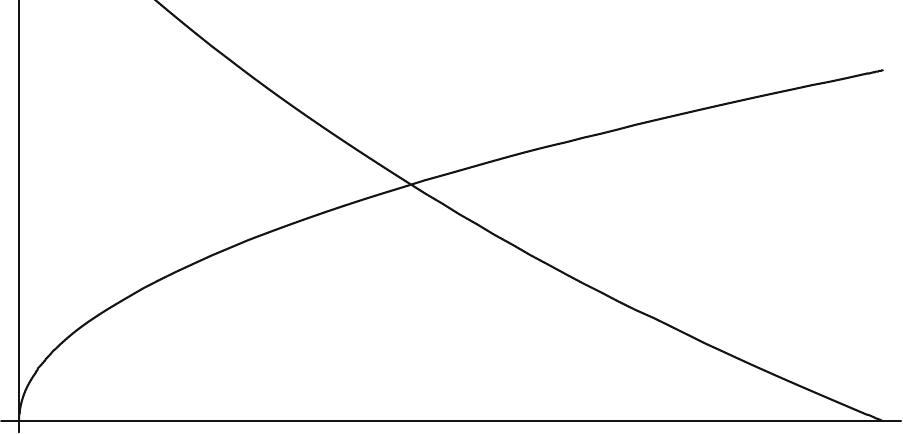
\includegraphics[width=.72\textwidth]{figures/figure-5-2.png}
  \caption{求解匹配条件:情形 1.}
  \label{fig:square-well-matching-case1}
\end{figure}

\begin{figure}[htbp]
  \centering
  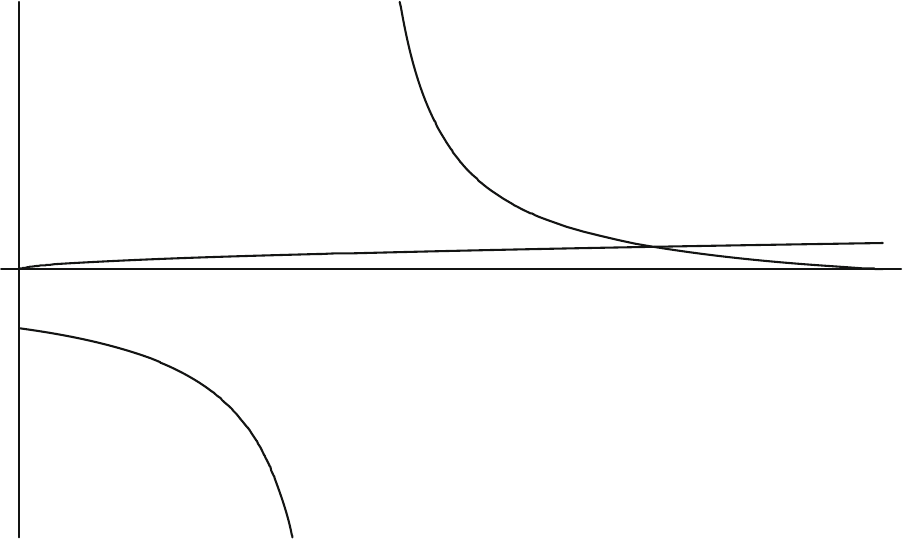
\includegraphics[width=.72\textwidth]{figures/figure-5-3.png}
  \caption{求解匹配条件:情形 2a.}
  \label{fig:square-well-matching-case2a}
\end{figure}

\begin{figure}[htbp]
  \centering
  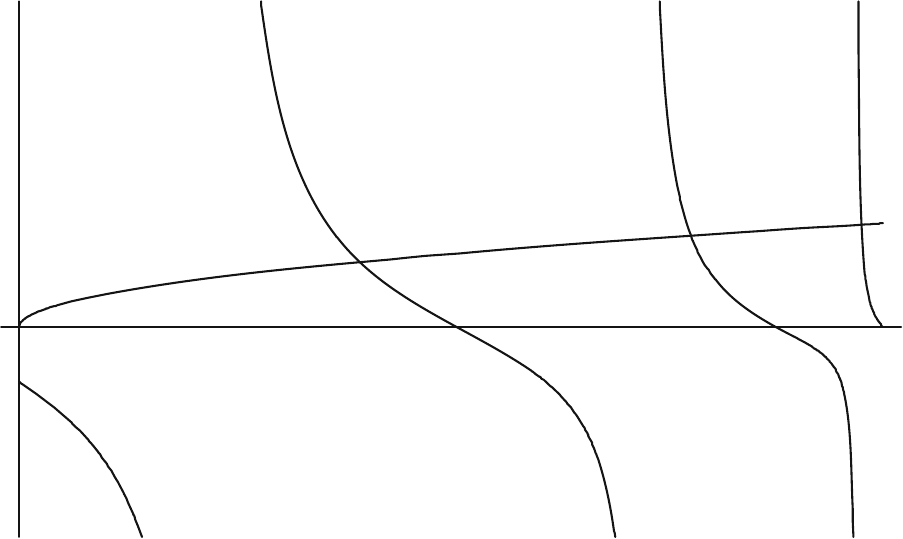
\includegraphics[width=.72\textwidth]{figures/figure-5-4.png}
  \caption{求解匹配条件:情形 2b.}
  \label{fig:square-well-matching-case2b}
\end{figure}

因此,至少找到了一个满足匹配条件的 \(\psi\),它和 \(\psi''\) 都在无穷远处指数衰减.由于该 \(\psi\) 属于 \(\widehat H\) 的定义域,得到如下结果.

\begin{proposition}[方势阱中的偶特征函数]\label{prop:square-well-even-eigenfunction}
对任意正数 \(A,C\),至少存在一个 \(E\in(-C,0)\),使得式~\eqref{eq:square-well-schrodinger} 在 \(\widehat H\) 的定义域中有非零解:
\[
\psi(x)=
\begin{cases}
\cos\left(\sqrt{c-\varepsilon}\,x\right),&-A\le x\le A,\\
\cos\left(\sqrt{c-\varepsilon}\,A\right)
\exp[-\sqrt{\varepsilon}(|x|-A)],&|x|\ge A,
\end{cases}
\]
其中 \(c,\varepsilon\) 由式~\eqref{eq:square-well-parameters} 定义,\(\varepsilon\) 满足式~\eqref{eq:square-well-even-matching}.
\end{proposition}

命题~\ref{prop:square-well-even-eigenfunction} 中没有把 \(\psi\) 归一化为 \(L^{2}(\mathbb{R})\) 中的单位向量,而是将 \(\psi\) 归一化为在原点取值 \(1\).图~\ref{fig:square-well-shallow-ground}--\ref{fig:square-well-deep-excited} 展示了几个例子.浅势阱(\(\sqrt c A=1\))只有一个偶特征向量,即系统基态(具有最小特征值的特征向量).对于深势阱(\(\sqrt c A=30\)),图中还展示了基态和一个激发态(特征值不是最小值的特征向量).

浅势阱中,基态在区间 \([-A,A]\) 外延伸得相当远;深势阱中,基态一离开势阱就很快趋于零.另一方面,图~\ref{fig:square-well-deep-excited} 中的激发态在势阱外延伸得相对较远.

\begin{figure}[htbp]
  \centering
  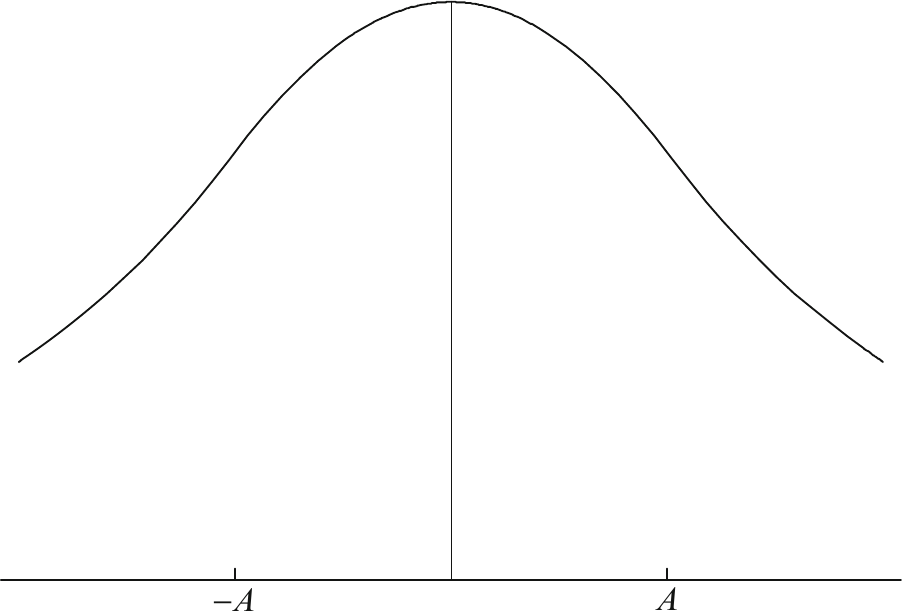
\includegraphics[width=.72\textwidth]{figures/figure-5-5.png}
  \caption{浅势阱的基态.}
  \label{fig:square-well-shallow-ground}
\end{figure}
\begin{figure}[htbp]
  \centering
  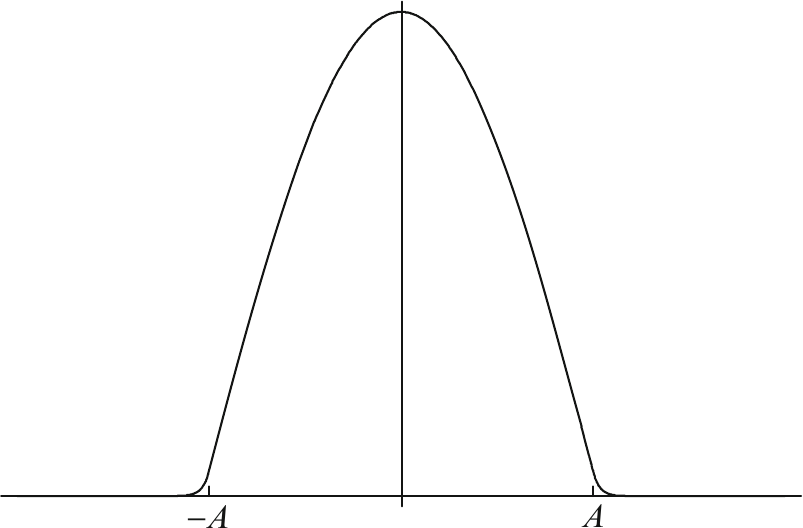
\includegraphics[width=.72\textwidth]{figures/figure-5-6.png}
  \caption{深势阱的基态.}
  \label{fig:square-well-deep-ground}
\end{figure}
\begin{figure}[htbp]
  \centering
  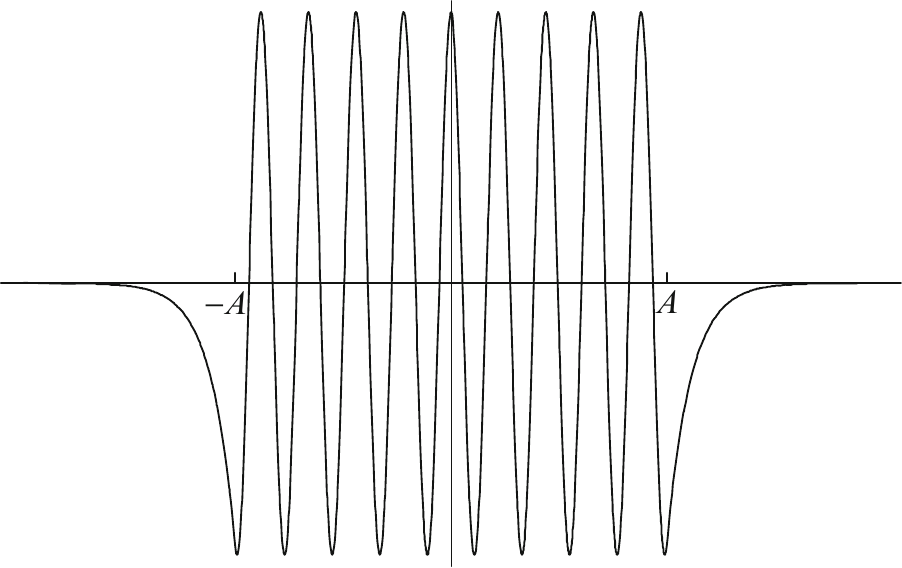
\includegraphics[width=.72\textwidth]{figures/figure-5-7.png}
  \caption{深势阱的激发态.}
  \label{fig:square-well-deep-excited}
\end{figure}

奇解的分析与上述类似.匹配条件~\eqref{eq:square-well-even-matching} 替换为
\begin{equation}
\sqrt{\varepsilon}
=-\sqrt{c-\varepsilon}\cot\left(\sqrt{c-\varepsilon}\,A\right),
\label{eq:square-well-odd-matching}
\end{equation}
(见练习~\ref{ex:square-well-odd-matching}),特征函数公式变为
\[
\psi(x)=
\begin{cases}
\sin\left(\sqrt{c-\varepsilon}\,x\right),&-A\le x\le A,\\
\pm\sin\left(\sqrt{c-\varepsilon}\,A\right)
\exp[-\sqrt{\varepsilon}(|x|-A)],&|x|\ge A,
\end{cases}
\]
其中 \(x>A\) 取正号,\(x<-A\) 取负号.

如果 \(\sqrt c A<\pi/2\),则式~\eqref{eq:square-well-odd-matching} 没有解,因为当 \(\varepsilon\in(0,c)\) 时右端始终为负.当 \(\sqrt c A\) 很大时,式~\eqref{eq:square-well-odd-matching} 会有多个解.典型的匹配情形和相应特征函数见图~\ref{fig:square-well-odd-matching} 与图~\ref{fig:square-well-odd-state}.

\begin{figure}[htbp]
  \centering
  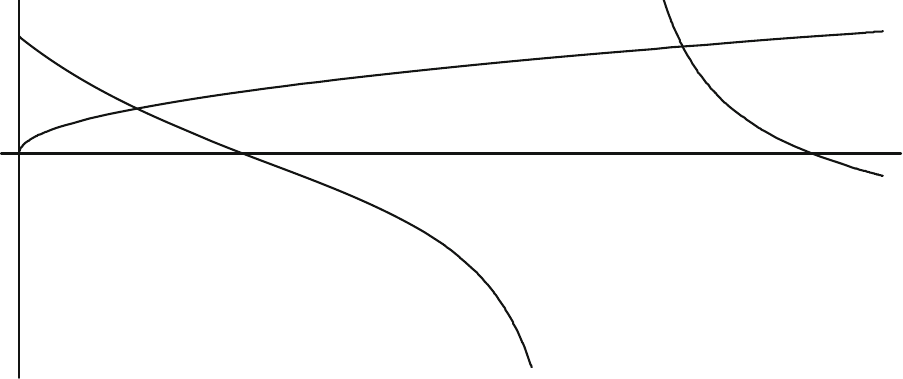
\includegraphics[width=.72\textwidth]{figures/figure-5-8.png}
  \caption{奇解的匹配条件.}
  \label{fig:square-well-odd-matching}
\end{figure}
\begin{figure}[htbp]
  \centering
  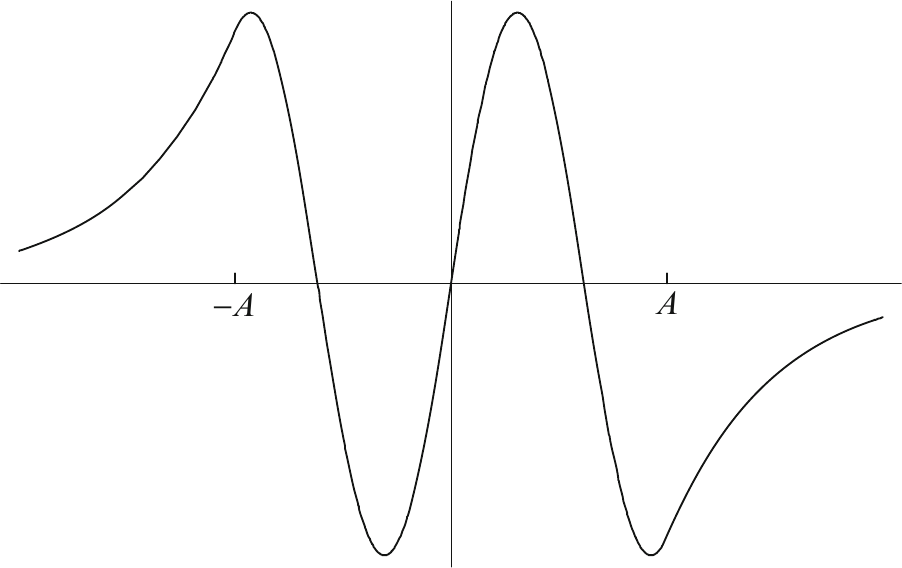
\includegraphics[width=.72\textwidth]{figures/figure-5-9.png}
  \caption{一个奇解.}
  \label{fig:square-well-odd-state}
\end{figure}

\section{隧穿与经典禁戒区域}\label{sec:tunneling}

简要比较经典情形与量子情形.经典地,如果粒子能量为 \(E\),由于动能 \(p^{2}/(2m)\) 总是非负,粒子不可能位于满足 \(V(x)>E\) 的点.于是 \(V(x)\le E\) 的区域称为“经典允许区域”,\(V(x)>E\) 的区域称为“经典禁戒区域”.对方势阱~\eqref{eq:square-well-potential},若 \(-C<E<0\),势阱本身(\(-A\le x\le A\) 的区域)是经典允许区域,而势阱外(\(|x|>A\))是经典禁戒区域.

量子地,若 \(\widehat H\psi=E\psi\),粒子具有确定能量 \(E\).然而,这样的粒子在经典禁戒区域内被发现的概率非零.注意,波函数在经典禁戒区域内虽然不为零,却随其到经典允许区域的距离指数衰减.换言之,量子粒子可以穿透一段距离进入经典禁戒区域.不过,如果 \(E\) 远小于零,即 \(\varepsilon\) 很大,那么满足 \(\widehat H\psi=E\psi\) 的状态在势阱外衰减得非常快,类似于 \(\exp[-\sqrt{\varepsilon}(|x|-A)]\).

更一般地,可以考虑能量近似为 \(E\) 的粒子的含时 Schrödinger 方程.如果要求能量严格等于 \(E\),那么时间依赖并不有趣,因为含时方程的解只是在时间上乘以一个常数相位.可是,我们可以考虑能量不确定度非零但很小的粒子.设粒子在 \(V<E\) 的区域内运动,随后接近 \(V>E\) 的区域(“势垒”).经典地,粒子会从势垒反射并返回;量子地,粒子却可能“隧穿”过势垒,在另一侧出现.也就是说,在稍后的某个时刻,波函数在势垒远侧会有一部分不可忽略的量.

\section{离散谱与连续谱}\label{sec:discrete-continuous-spectrum}

我们对 \(-C<E<0\) 范围内特征值方程~\eqref{eq:square-well-schrodinger} 的分析表明,只有有限多个 \(E\) 值能产生平方可积解.分析 \(E\le-C\) 的情形不难得到:所有非零解至少在一个方向上指数增长(见练习~\ref{ex:square-well-no-low-states}).另一方面,当 \(E>0\) 时,\((-\infty,-A)\) 上的任何解都具有正弦式行为,除非恒等于零,否则不平方可积;根据匹配条件,此时解必须处处为零.

因此,式~\eqref{eq:square-well-schrodinger} 只有有限多个平方可积解(每个解都只确定到常数倍).显然,真正的特征向量——即实际属于 Hilbert 空间 \(L^{2}(\mathbb{R})\) 的特征向量——不可能构成 \(L^{2}(\mathbb{R})\) 的标准正交基.不过,谱定理(第~7 章)会提供某种类似于标准正交基分解的表达,把 \(L^{2}(\mathbb{R})\) 中的元素用式~\eqref{eq:square-well-schrodinger} 的解表示.\(L^{2}(\mathbb{R})\) 中的一般元素 \(\psi\) 是两项之和:第一项是 \(\widehat H\) 的真正(\(L^{2}\))特征向量(它们的 \(E<0\))的线性组合;第二项是 \(E>0\) 的不可平方积“广义特征向量”的连续叠加,即积分.

第~9 章将引入(可能无界的)自伴算子 \(A\) 的谱概念:若对每个 \(\varepsilon>0\),都存在 \(A\) 定义域中的单位向量 \(\psi\),使得 \(\|A\psi-\lambda\psi\|<\varepsilon\),则数 \(\lambda\) 属于 \(A\) 的谱.对方势阱的 Hamilton 算子 \(\widehat H\),不难证明每个满足 \(E\ge0\) 的实数都属于 \(\widehat H\) 的谱(见练习~\ref{ex:square-well-spectrum-positive}).

还可以证明,如果 \(E<0\) 不是特征值(即 \(\widehat H\psi=E\psi\) 没有非零 \(L^{2}\) 解),那么 \(E\) 不属于 \(\widehat H\) 的谱.练习~\ref{ex:square-well-spectrum-negative} 暗示了这一结果.因此,\(\widehat H\) 的谱由 \((-C,0)\) 中的有限个点(至少一个)和整个半轴 \([0,\infty)\) 组成.

\section{练习}\label{sec:chapter5-exercises}

\begin{exercise}\label{ex:square-well-domain-distribution}
\begin{enumerate}
\item 设 \(\psi\) 在 \((-\infty,-A)\)、\((-A,A)\) 和 \((A,\infty)\) 上分别光滑,并在 \(x=A\) 与 \(x=-A\) 处 \(\psi,\psi'\) 都连续.证明对任意紧支集光滑函数 \(\chi\),有
\[
\int_{-\infty}^{\infty}\chi''(x)\psi(x)\,\mathrm{d}x
=\int_{-\infty}^{\infty}\chi(x)\psi''(x)\,\mathrm{d}x,
\]
其中若 \(\psi''\) 在 \(x=\pm A\) 处不存在,则不定义这两个点处的 \(\psi''\).(根据定义~\ref{app:def:distribution-derivative},这意味着 \(\psi\) 的分布二阶导数就是函数 \(\psi''\).)提示:取包含 \(\chi\) 支集的区间 \([-R,R]\),其中 \(R>A\),然后分别在 \([-R,-A]\)、\([-A,A]\) 和 \([A,R]\) 上分部积分,并仔细处理边界项.
\item 现在设 \(\psi\) 在上述三个区间上分别光滑,并且 \(\psi,\psi'\) 在 \(x=\pm A\) 处有左右极限,但假设 \(\psi'\) 在 \(x=-A\) 处有间断.证明上式右端必须增加 \(\chi(-A)\) 的某个非零倍数.
\end{enumerate}
\end{exercise}

\begin{exercise}\label{ex:square-well-odd-matching}
验证定态 Schrödinger 方程奇解的匹配条件~\eqref{eq:square-well-odd-matching}.
\end{exercise}

\begin{exercise}\label{ex:square-well-oscillatory}
设 \(\omega\) 是非零实数,\(\psi(x)=a\cos(\omega x)+b\sin(\omega x)\),其中 \(a,b\) 为实数且不同时为零.证明对任意 \(A\in\mathbb{R}\),有
\[
\lim_{B\to+\infty}\int_{A}^{B}\psi(x)^{2}\,\mathrm{d}x=+\infty.
\]
\end{exercise}

\begin{exercise}\label{ex:square-well-spectrum-positive}
设 \(f\) 是区间 \((0,1)\) 上的 \(C^{\infty}\) 函数,且 \(0<x<1/3\) 时 \(f(x)=1\),\(2/3<x<1\) 时 \(f(x)=0\).在 \(\mathbb{R}\) 上定义“截断”函数族 \(\chi_{n}\):
\[
\chi_{n}(x)=
\begin{cases}
0,&|x|\ge n+1,\\
1,&|x|\le n,\\
f(-x-n),&-(n+1)<x<-n,\\
f(x-n),&n<x<n+1.
\end{cases}
\]
给定 \(E>0\),设 \(\psi\) 是式~\eqref{eq:square-well-schrodinger} 的非零解,且 \(\psi,\psi'\) 在 \(x=\pm A\) 连续.令 \(\psi_{n}=\psi\chi_{n}\).证明 \(\psi_{n}\) 属于 \(\widehat H\) 的定义域,并且
\[
\lim_{n\to\infty}\frac{\|\widehat H\psi_{n}-E\psi_{n}\|}{\|\psi_{n}\|}=0.
\]
\begin{note}
第~9 章将看到,这意味着每个 \(E>0\) 的实数都属于算子 \(\widehat H\) 的谱.
\end{note}
\begin{solution}
估计分子时使用 \(\chi_n'\) 和 \(\chi_n''\) 只支集在两个过渡区间这一事实;估计分母时可对 \(\psi\) 的实部和虚部分别使用练习~\ref{ex:square-well-oscillatory}.
\end{solution}
\end{exercise}

\begin{exercise}\label{ex:square-well-spectrum-negative}
设 \(E<0\),并假设式~\eqref{eq:square-well-schrodinger} 不存在 \(\psi,\psi'\) 连续的非零平方可积解.令 \(\psi\) 是 \(\psi,\psi'\) 在 \(x=\pm A\) 连续的非零解,令 \(\psi_n\) 如练习~\ref{ex:square-well-spectrum-positive}.证明
\[
\frac{\|\widehat H\psi_{n}-E\psi_{n}\|}{\|\psi_{n}\|}
\]
不趋于零.
\end{exercise}

\begin{exercise}\label{ex:square-well-no-low-states}
\begin{enumerate}
\item 证明,当 \(E<-C\) 时,式~\eqref{eq:square-well-schrodinger} 不存在 \(\psi,\psi'\) 连续的非零平方可积解.
\item 对 \(E=-C\) 得到同样的结论.
\end{enumerate}
\begin{note}
分别分析偶解与奇解.
\end{note}
\end{exercise}

\begin{exercise}\label{ex:square-well-ground-state}
把方势阱中粒子的基态定义为具有最低(最负)特征值的特征向量,它对应于最大的 \(\varepsilon\) 值.
\begin{enumerate}
\item 证明基态总是偶函数,即证明满足式~\eqref{eq:square-well-even-matching} 的最大 \(\varepsilon\) 总大于式~\eqref{eq:square-well-odd-matching} 的任何解.
\item 证明基态是处处非零的函数.
\end{enumerate}
\end{exercise}
